Per avviare una presentazione è necessario prima selezionare il progetto dalla lista dei progetti disponibili. Una volta selezionato il progetto, apparirà al centro dello schermo il titolo del progetto scelto, un'immagine di default e sotto a questa un menù. Selezionando dal menù la voce \textbf{Play} si aprirà una nuova scheda nel browser\ped{G} dove sarà avviata la presentazione.

\begin{figure}[H] 
	\centering 
	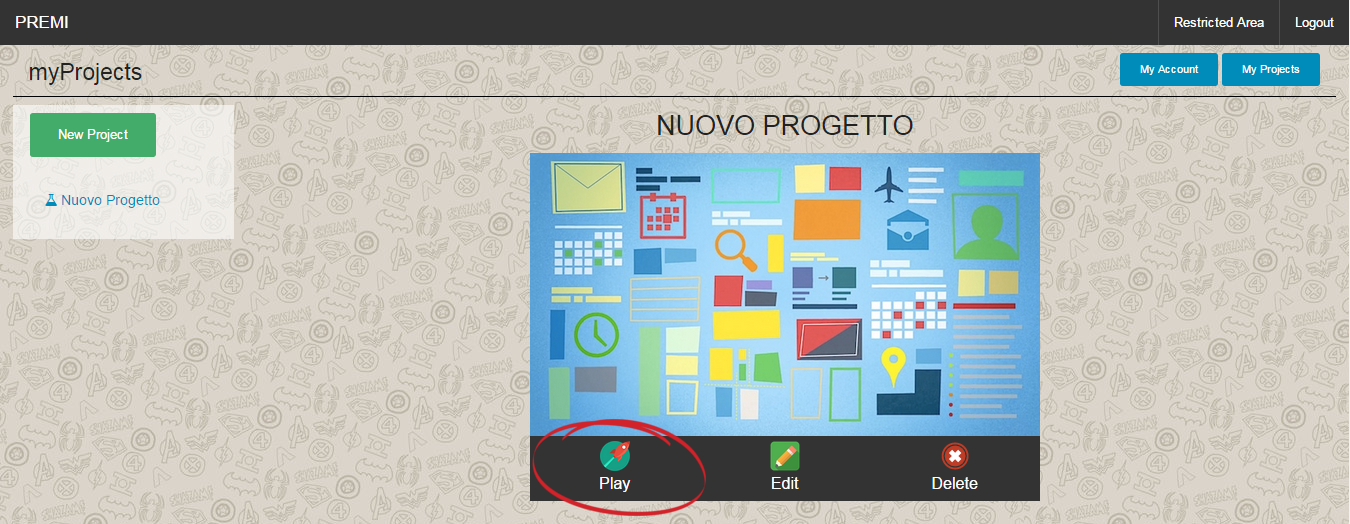
\includegraphics[scale=0.40] {img/avv_pres.png}
	\caption{Avvio di una presentazione} 
\end{figure}

\subsection{Menù di navigazione}
\noindent Il menù di navigazione è composto da quattro frecce di colore diverso in base alle slide\ped{G} che sono disponibili nella direzione indicata dalla freccia e dal numero di pagina corrente della slide\ped{G}. Se la freccia è di colore trasparente non ci sono slide\ped{G} disponibili in quella direzione, viceversa se la freccia è di colore blu ci si può spostare in quella direzione verso la prossima slide\ped{G}. Come esempio si prenda l'immagine sottostante, che indica la possibilità di visualizzare la prossima slide spostandosi a sinistra o in basso.

\begin{figure}[H] 
	\centering 
	
\includegraphics[scale=0.70] {img/nav.png}
	\caption{Menù di navigazione in dettaglio} 
	\end{figure}

\subsection{Presentazione in modalità ascoltatore}

\noindent Una volta avviata una presentazione essa verrà avviata di automaticamente in modalità ascoltatore. Verrà visualizzata la prima slide\ped{G} del progetto e, in basso a destra, il menù di navigazione utilizzabile sia con il mouse sia con i tasti freccia della tastiera. Inoltre in basso e per tutta la lunghezza dello schermo si trova una piccola barra blu che indica l'avanzamento della presentazione: man mano che si procede con la presentazione essa si sposta verso destra.
\begin{figure}[H] 
	\centering 
	
\includegraphics[scale=0.40] {img/sfondook.png}
	\caption{Presentazione in modalità ascoltatore} 
\end{figure}


\subsection{Presentazione in modalità presentatore}
\noindent Per avviare presentazione in modalità presentatore è necessario avviare prima una presentazione come ascoltatore. Una volta avviata è necessario premere il tasto \textbf{S} della tastiera per avviare la modalità presentatore.
\begin{figure}[H] 
	\centering 
	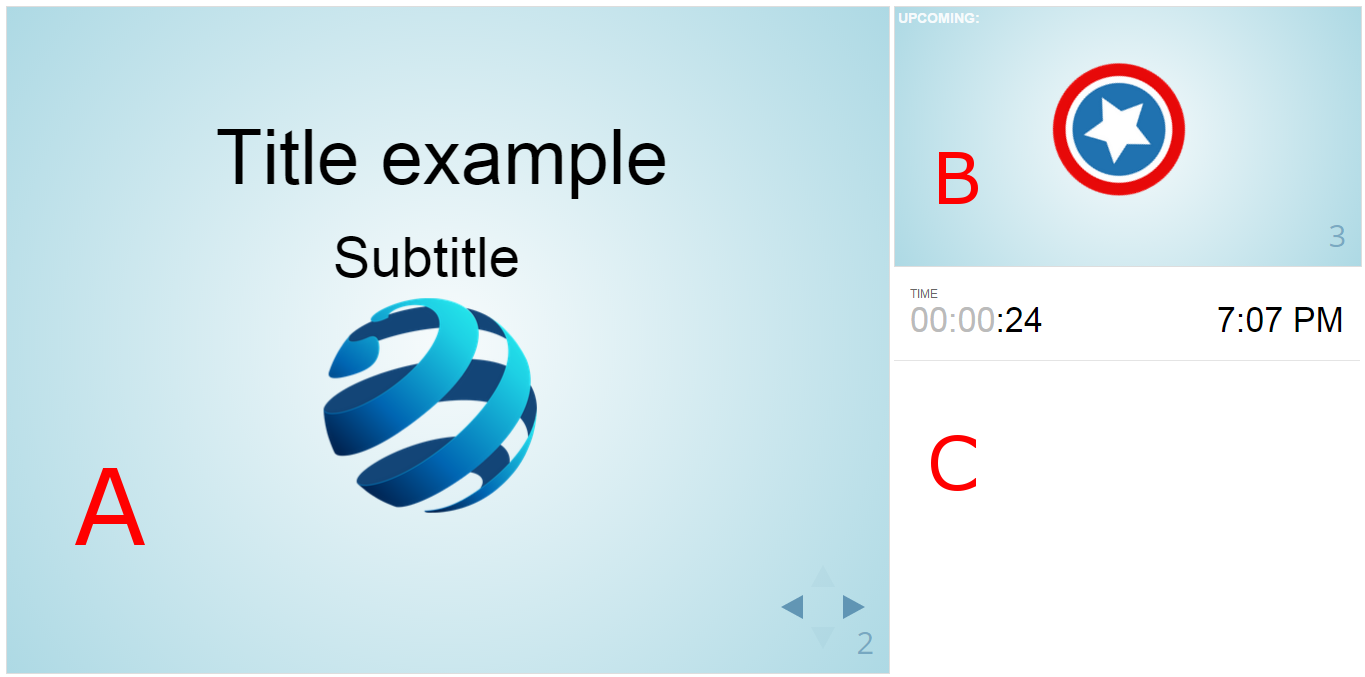
\includegraphics[scale=0.40] {img/note.png}
	\caption{Presentazione in modalità presentatore} 
\end{figure}

\noindent Come si può notare dall'immagine precedente, l'interfaccia grafica di questa modalità presenta delle funzionalità di supporto al presentatore, dividendo lo schermo in tre parti ben distinte:
\begin{itemize}
	\item \textbf{A}: in questa parte di schermo viene visualizzata la slide\ped{G} che attualmente si sta visualizzando;
	\item \textbf{B}: in questa parte di schermo viene visualizzata la prossima slide\ped{G} che verrà visualizzata;
	\item \textbf{C}: in questa parte di schermo vengono visualizzati gli aiuti al presentatore, cioè il tempo trascorso da quando la presentazione è partita e l'orario corrente. Se si effettua un click con il tasto sinistro del mouse sul timer questo si resetta.
\end{itemize}

\subsection{Scorciatoie da tastiera}
\noindent Una volta avviata una presentazione, in qualunque modalità, sono possibili le seguenti azioni:
\begin{itemize}
	\item \textbf{Tasto ESC}: la pressione di questo tasto permette la visualizzazione della matrice completa di tutte le slide\ped{G} che compongono la presentazione. Ripremendo il tasto \textbf{ESC} si ritorna alla visualizzazione normale delle slide\ped{G};
	\begin{figure}[H] 
		\centering 
		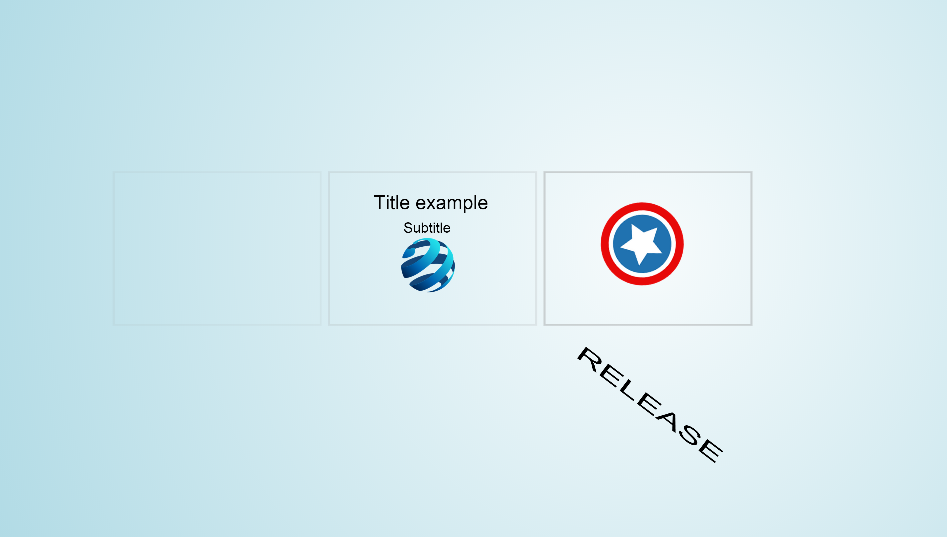
\includegraphics[scale=0.40] {img/anteprima.png}
		\caption{Tasto ESC - Matrice delle slide} 
	\end{figure}
	\item \textbf{Tasto B}: la pressione di questo tasto permette di mettere in pausa la presentazione oscurando la slide\ped{G} corrente. Per riprendere la presentazione è sufficiente ripremere il tasto \textbf{B}.
	\begin{figure}[H] 
		\centering 
		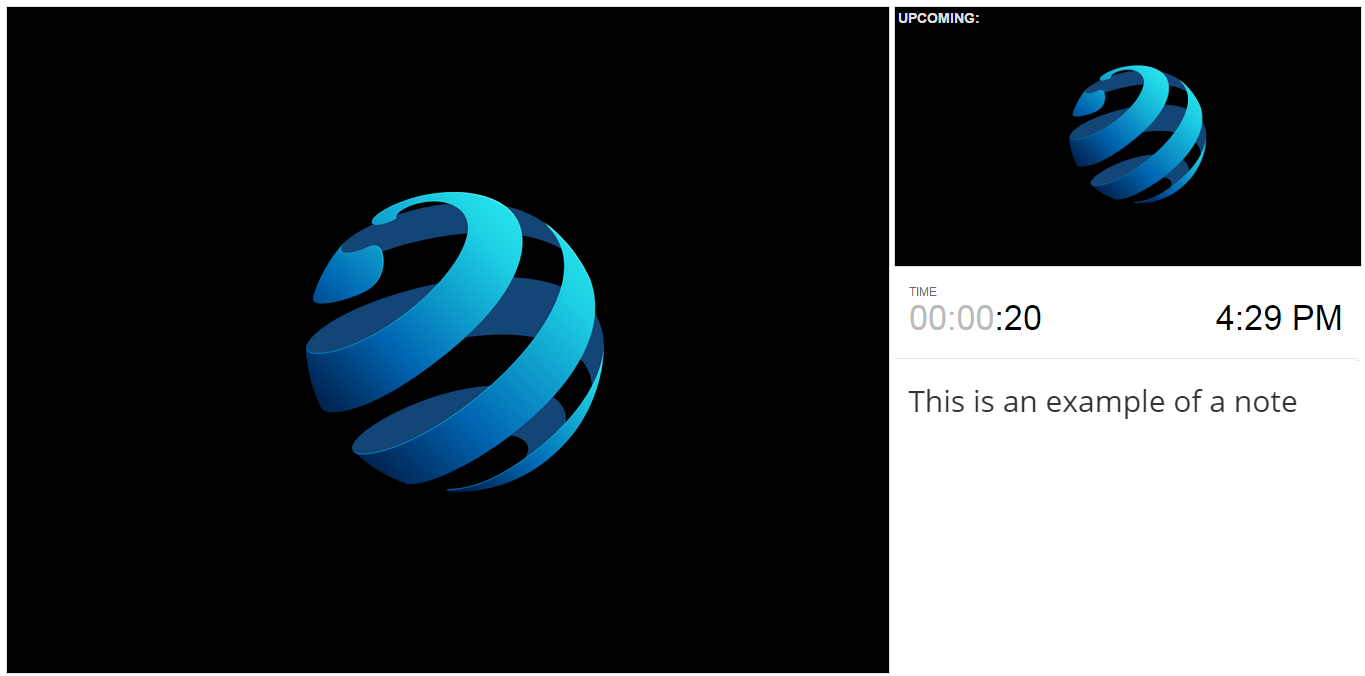
\includegraphics[scale=0.20] {img/b.png}
		\caption{Tasto B - Pausa della presentazione in modalità ascoltatore} 
	\end{figure}
	
	\begin{figure}[H] 
		\centering 
		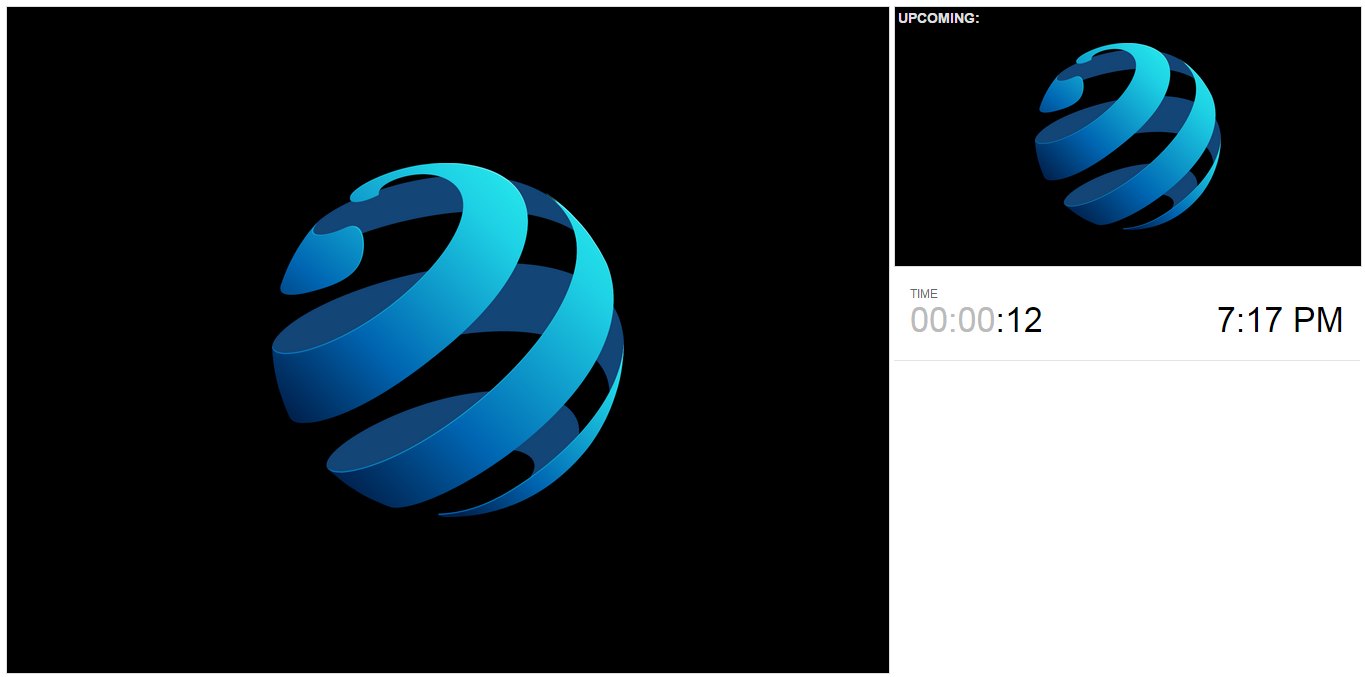
\includegraphics[scale=0.30] {img/b1.png}
		\caption{Tasto B - Pausa della presentazione in modalità presentatore} 
	\end{figure}
\end{itemize}
